\documentclass[12pt,a4paper]{article}


%%%%%%%%%%%% Package %%%%%%%%%%%
\usepackage{etex}
\usepackage{xfakebold} %Pour le gras
\usepackage{esvect}
\usepackage[utf8]{inputenc}
\usepackage[french]{babel}
\usepackage[autolanguage]{numprint} % Pour écrire les nombres comme dans la langue du text
\usepackage[T1]{fontenc}
\usepackage{amsmath,amssymb,amsfonts, amsthm}
\usepackage{systeme} 
\usepackage{empheq,etoolbox}
\usepackage{array}
\usepackage{nicematrix}
\usepackage{enumitem}
\usepackage{mathrsfs}
\usepackage{mathtools}
\usepackage{cancel}
\usepackage{wrapfig}
\usepackage{stmaryrd}
\usepackage{bbm}
\usepackage{booktabs}
% Interligne
\usepackage{setspace}
\usepackage{verbatim}
% \singlespacing
%\onehalfspacing
% \doublespacing
\usepackage{multirow, multicol}
\usepackage{adjustbox}
\usepackage{cite}
\usepackage{titlesec}

\usepackage{listings}
\usepackage[framed, numbered]{matlab-prettifier}




%%%%%% Geometry %%%%%%%
\usepackage{geometry}
\geometry{left=1.5cm,right=1.5cm,top=2cm,bottom=2cm}
\savegeometry{1}

\geometry{left=1cm,right=1cm,top=2.7cm,bottom=1.4cm}
\savegeometry{2}

\geometry{left=2.5cm,right=2.5cm,top=3cm,bottom=3cm}
\savegeometry{3}

%%%%%%%%%%%%%%%%%%%%%%%%

\usepackage{graphicx,mwe,fancyhdr}
\usepackage{fancybox}
\usepackage{siunitx}
\sisetup{locale = FR,
	detect-all,range-phrase=-,     
	range-units=single,
	separate-uncertainty = true,
	multi-part-units = single
}
\usepackage{lmodern}
\usepackage{hyperref}
\hypersetup{colorlinks=true}
%\hypersetup{final}
\usepackage{tabularx}
\usepackage{color,xcolor}
\usepackage[table]{}
\definecolor{dkgreen}{rgb}{0,0.6,0}
\definecolor{gray}{rgb}{0.5,0.5,0.5}
\definecolor{mauve}{rgb}{0.58,0,0.82}

\setlength{\arrayrulewidth}{.5mm}
%\arrayrulecolor{blue}

\usepackage[most]{tcolorbox}

%%%%% Graphique %%%%%%%%
%\usepackage{tikz}
	\usepackage{tikz-network}       % Pour la théorie des graphes (vertices & edges)
	
	\tikzset{>=stealth}
	\usepackage{pgfplots,pgfplotstable}
	%\usepackage[miktex]{gnuplottex}
	\pgfkeys{/pgf/number format/1000 sep={\,}, /pgf/number format/use comma,  } % Pour avoir des virgules au lieu des points comme séparateur décimal dans les Axes graph
	%\pgfkeys{/pgf/plot/gnuplot call='C:\Program Files\gnuplot\bin\gnuplot'}
	\pgfplotsset{compat=newest}
	\usepackage{mathrsfs}
	\usepgfplotslibrary{groupplots}
	\usetikzlibrary{shapes.geometric, shapes.misc, intersections,calc, arrows}
	\lstset{ %
		language=R,                     % the language of the code
		basicstyle=\footnotesize,       % the size of the fonts that are used for the code
		numbers=left,                   % where to put the line-numbers
		numberstyle=\tiny\color{gray},  % the style that is used for the line-numbers
		stepnumber=1,                   % the step between two line-numbers. If it's 1, each line
		% will be numbered
		numbersep=5pt,                  % how far the line-numbers are from the code
		backgroundcolor=\color{white},  % choose the background color. You must add \usepackage{color}
		showspaces=false,               % show spaces adding particular underscores
		showstringspaces=false,         % underline spaces within strings
		showtabs=false,                 % show tabs within strings adding particular underscores
		%frame=single,                   % adds a frame around the code
		rulecolor=\color{black},        % if not set, the frame-color may be changed on line-breaks within not-black text (e.g. commens (green here))
		tabsize=2,                      % sets default tabsize to 2 spaces
		captionpos=b,                   % sets the caption-position to bottom
		breaklines=true,                % sets automatic line breaking
		breakatwhitespace=false,        % sets if automatic breaks should only happen at whitespace
		title=\lstname,                 % show the filename of files included with \lstinputlisting;
		% also try caption instead of title
		keywordstyle=\color{blue},      % keyword style
		commentstyle=\color{dkgreen},   % comment style
		stringstyle=\color{mauve},      % string literal style
		escapeinside={\%*}{*)},         % if you want to add a comment within your code
		morekeywords={*,...}            % if you want to add more keywords to the set
	} 
\usetikzlibrary{matrix}


%%%%%%% Commandes Perso %%%%%%%%
\DeclarePairedDelimiter\floor{\lfloor}{\rfloor}
\DeclareMathOperator{\Ham}{\mathcal{H}}	% Opérateur hamiltonien
\DeclareMathOperator*{\argmax}{argmax} % Les antecedants du max
\DeclareMathOperator*{\argmin}{argmin} % Les antecedants du max
\DeclareMathOperator{\sinc}{\text{sinc}} % sinus cardinal
\DeclareMathOperator{\erfc}{\text{erfc}}
\renewcommand{\Re}{\text{Re}}			 % Partie réelle
\DeclareMathOperator{\sgn}{\text{sgn}}	 % Fonction signe
\DeclareMathOperator{\e}{\text{e}}		 % L'opérateur exponentiel e
\DeclareSIUnit{\baud}{\text{baud}}
\DeclareSIUnit{\sym}{\text{sym}}
\newcommand{\iu}{\mathrm{i}}			 % i imaginaire complexe
\newcommand{\deriv}{\text{d}}			 % le d de la différenciabilité
\newcommand{\ens}[1]{\mathbb{#1}}              					%Ensemble usuelle : N, Z, R, C, Q, K
\newcommand{\abs}[1]{\left\vert {#1}\right\vert}				%Valeur absolue
\newcommand{\partiel}[2]{\frac{\partial {#1}}{\partial {#2}}}	%derivée partielle
\newcommand{\pesp}{\,}											%petit espace
\newcommand{\gesp}{\;}											%grand espace
\newcommand{\nesp}{\˽}											%normal espace
\newcommand{\grandm}{\displaystyle}								%grande écriture maths
\newcommand{\petitm}{\scriptstyle}								%petite écriture maths
\newcommand{\im}[1]{\text{Im}\,{#1}}							%Ensemble image
\newcommand{\Ker}[1]{\text{Ker}\,{#1}}							%Noyau ou Ker
\newcommand{\somme}[2]{\overset{#2}{\underset{#1}{\sum}} \,}	%Operateur de sommation
%\newcommand{\norm}[1]{\left\Vert #1\right\Vert}
\newcommand{\norm}[1]{\left\|{#1}\right\|}						%Norme vectorielle avec 2 barres
\newcommand{\fonctnorm}[1]{{\left\vert\kern-0.25ex\left\vert\kern-0.25ex\left\vert #1 % Norme fonctionnelle avec 3 barres
		\right\vert\kern-0.25ex\right\vert\kern-0.25ex\right\vert}}
\newcommand{\ensvide}{\varnothing}								%Ensemble vide
\newcommand{\limite}[1]{\lim\limits_{#1}}						%Operateur de limite
\newcommand{\boule}[2]{\mathcal{B}\left({#1},{#2}\right)}		%Boule avec centre et rayon
\newcommand{\boulef}[2]{\overline{\mathcal{B}}\left({#1},{#2}\right)} %Boule fermée 
\newcommand{\sphere}[2]{\mathcal{S}\left({#1},{#2}\right)} 				%Sphere avec centre et rayon
\newcommand{\spheref}[2]{\overline{\mathcal{S}}\left({#1},{#2}\right)} 
\newcommand{\disqf}[2]{\overline{\mathcal{D}}\left({#1},{#2}\right)}	%Disque fermée
\newcommand{\disq}[2]{\mathcal{D}\left({#1},{#2}\right)}				%Disque ouvert
\newcommand{\dif}[2]{\mathrm{d}_{#2}{#1}}								%Différentielle d'une fonction en un point
\newcommand{\Vecteur}[1]{\boldsymbol{\mathbf{#1}}}						%Vecteur gras
\newcommand{\jac}[2]{J_{#2} #1}											%Jacobienne d'une fonction en un point
\newcommand{\transp}[1]{{}^\text{t}\! #1}								%La transposée
\newcommand{\prdtscal}[2]{\langle #1, #2\rangle} 						%Produit scalaire
\newcommand{\flux}[2]{\Phi_{{#1}\rightarrow{#2}}}						%Flux d'un champs le long d'une surface
\newcommand{\ensemble}[2]{\left\lbrace   #1\; \left|\; #2 \right\rbrace  \right.} %Ensemble en compréhension
\renewcommand*{\overrightarrow}[1]{\vbox{\halign{##\cr 
			\tiny\rightarrowfill\cr\noalign{\nointerlineskip\vskip1pt} 
			$#1\mskip2mu$\cr}}}
\newcommand{\vecteur}[1]{\overrightarrow{#1}\hspace*{-2pt}}							%Vecteur avec une grande fleche
\newcommand{\Int}[4]{\int_{#1}^{#2} {#3} \mathrm{d}#4}					%Intégrale
\renewcommand{\thefootnote}{(\alph{footnote})}	
\DeclareMathOperator{\rot}{\vecteur{\text{rot}}} 						% Rotationnel
\DeclareMathOperator{\divergence}{\mathrm{div}}						% Divergence
\DeclareMathOperator{\gradient}{\vecteur{\mathrm{grad}}}				% Gradient

%%%%%% Definition de la gaussienne pour PGF %%%%%
\pgfmathdeclarefunction{gauss}{2}{%
	\pgfmathparse{1/(#2*sqrt(2*pi))*exp(-((x-#1)^2)/(2*#2^2))}%
}
%% variable de gauss(<moyenne>,<ecart-type>)


\pgfplotsset{
	legend entry/.initial=,
	every axis plot post/.code={%
		\pgfkeysgetvalue{/pgfplots/legend entry}\tempValue
		\ifx\tempValue\empty
		\pgfkeysalso{/pgfplots/forget plot}%
		\else
		\expandafter\addlegendentry\expandafter{\tempValue}%
		\fi
	},
}



\newcommand*{\colorboxed}{}
\def\colorboxed#1#{%
	\colorboxedAux{#1}%
}
\newcommand*{\colorboxedAux}[3]{%
	% #1: optional argument for color model
	% #2: color specification
	% #3: formula
	\begingroup
	\colorlet{cb@saved}{.}%
	\color#1{#2}%
	\boxed{%
		\color{cb@saved}%
		#3%
	}%
	\endgroup
}

\setlength{\fboxrule}{0.3mm}

%\setBold[0.2] % Active la police grasse 

%%%%%%%%% Environnement Perso %%%%%%%%
\theoremstyle{definition}	 %Garde la même police pour l'environnement 
\newtheorem{questo}{Question}[section] % Création de l'environnement exo dont le numérotage est indépendant des autres environnement
\newtheorem{manip}{Manipulation}[section] % Création de l'environnement question dont le numerotage depend de l'environnement exo
\pagestyle{plain} 

%%%%%%%%% Environnement Tcolor Perso %%%%%%%%
\newtcbtheorem{tquesto}{Question}{colback=blue!5, colframe=blue!60!black}{}
\newtcbtheorem[number within = section]{tmanip}{Manipulation}{colback=red!5, colframe=red!60!black}{}




\numberwithin{equation}{section}
\numberwithin{figure}{section}

% \usepgfplotslibrary{external}
% \tikzexternalize[prefix=./tikz/,optimize command away=\includepdf,shell escape=-enable-write18]
% \tikzset{external/system call= {pdflatex -save-size=80000 
%                           -pool-size=10000000 
%                           -extra-mem-top=50000000 
%                           -extra-mem-bot=10000000 
%                           -main-memory=90000000 
%                           \tikzexternalcheckshellescape 
%                           -halt-on-error 
%                           -interaction=batchmode
%                           -jobname "\image" "\texsource"}}

%\setBold[0.2] % Active la police grasse 
\title{\textsc{Machine Learning LAB - Optimal binary Bayesian classifer}}
\author{Mahamat HAMID \and Yassine KADDAMI}
%\date{October 2022}

\begin{document}
	\loadgeometry{1}
	\maketitle
	%\tableofcontents
	%\newpage
	\section{Theoretical computations}
	The purpose of this lab is to study the MPE test and assess it with respect to the Neyman-pearson test.
Section 1 is dedicated to the theoretical computations that you are asked in Section 2 to implement so as
to run simulations and verify these theoretical results. All the results needed to write your routines, in
whatever language you wish to use, are given below; in Section 1.2, these results are framed. Hence, it is
suggested that you begin by carrying out the simulations of Section 2 and make the theoretical computations
later. You can return your theoretical computations in latex, word or even as a photo of your hand-writen
notes (if the writing and the presentation are clear).
\subsection{The MPE test and its probability of error}

We consider the binary hypothesis testing problem : 
$$ \begin{cases}
    \mathcal{H}_0 :\,  X \sim \mathcal{N}(0,\sigma^2 \textbf{I}_N) \\
    \mathcal{H}_1 :\,   X \sim \mathcal{N}(\theta,\sigma^2 \textbf{I}_N)
\end{cases} \quad \text{where }\sigma>0 \text{ and } \theta \in \ens{R}^N $$
 We assume the existence of prior probabilities of occurrence $\pi_0$ and $\pi_1$
for $\mathcal{H}_0$ and $\mathcal{H}_1,$ respectively. Alternatively, we can also pose : 
$$X = \varepsilon X_1 + (1-\varepsilon)X_0 $$
where $\varepsilon, X_0$ and $X_1$ are random variables defined in same probability space $(\Omega, \Sigma, \ens{P})$ such that :

\begin{itemize}[label = $\bullet$]
    \item $ X_0 \sim \mathcal{N}(0,\sigma^2 \textbf{I}_N) $ and $X_1 \sim \mathcal{N}(\theta,\sigma^2 \textbf{I}_N)$
    \item  $\varepsilon$ is independant of $X_1$ and  $X_0$
    \item  $\pi_0 = \ens{P}(\varepsilon = 0)$ and $\pi_1 =\ens{P}(\varepsilon = 1)$
\end{itemize}


\begin{tquesto}{}{}
Compute the likelihood ratio $\Lambda = p_1/p_0 $ of the two hypotheses where $p_1$ is the pdf of $X_1$ and $p_0$
that of $X_0$ (see slide 17) (\textbf{2 pts}).
\end{tquesto}

L'expression des densités de probabilités $p_1$ et $p_0$ est la suivante : 
 $$ \begin{cases}
     p_0(x) & = \dfrac{1}{(2\pi)^{N/2}\sqrt{\abs{\det\left( \sigma^2 \textbf{I}_N \right)}}}\exp\left\{ -\dfrac{1}{2\sigma^2} x^t \cdot \textbf{I}_N\cdot x \right\} \\

     p_1(x) & = \dfrac{1}{(2\pi)^{N/2}\sqrt{\abs{\det\left( \sigma^2 \textbf{I}_N \right)}}}\exp\left\{ -\dfrac{1}{2\sigma^2} (x-\theta)^t \cdot \textbf{I}_N\cdot (x-\theta) \right\} 
 \end{cases}$$
Ainsi en faisant le rapport on trouve : 

\begin{align*}
    \Lambda (x) & =  \dfrac{\exp\left\{ -\dfrac{1}{2\sigma^2} (x-\theta)^t \cdot \textbf{I}_N\cdot (x-\theta) \right\} } {\exp\left\{ -\dfrac{1}{2\sigma^2} x^t \cdot \textbf{I}_N\cdot x \right\}} \\ 
    & = \dfrac{\exp\left\{ -\dfrac{1}{2\sigma^2}\norm{x-\theta}^2 \right\}}{\exp\left\{ -\dfrac{1}{2\sigma^2}\norm{x}^2 \right\}} \\
    & = \exp\left\{  -\dfrac{1}{2\sigma^2}\left(\norm{x-\theta}^2 - \norm{x}^2\right) \right\} = \exp\left\{  -\dfrac{1}{2\sigma^2}\left(\cancel{\norm{x}^2} + \norm{\theta}^2 - 2x^t\cdot\theta - \cancel{\norm{x}^2}\right) \right\}
\end{align*}
 D'où : $$     \colorboxed{red}{\Lambda (x) =  \exp\left\{ \dfrac{1}{\sigma^2}\left(x^t\cdot \theta - \dfrac{\norm{\theta}^2}{2} \right)\right\}}$$

\begin{tquesto}{}{}
Show that the MPE classifier (see slides 16 and 17) is given by :
$$ \forall x \in \ens{R}^N,\quad g_\text{MPE}(x) = \begin{cases}
    1 &\text{ if } x^t\cdot\theta >\sigma^2\ln(\pi_0/\pi_1) + \norm{\theta}^2/2 \\
    0 & \text{ otherwise } 
\end{cases} $$
(\textbf{2 pts})
\end{tquesto}

 \begin{align*}
\pi_1 p_1(x) > \pi_0 p_0(x) & \Longleftrightarrow \dfrac{p_1}{p_0}(x) > \dfrac{\pi_0}{\pi_1} \quad\text{ si }\pi_1, p_0(x) \text{ non nuls} \\
 & \Longleftrightarrow \Lambda(x) > \dfrac{\pi_0}{\pi_1} \\
 & \Longleftrightarrow \exp\left\{ \dfrac{1}{\sigma^2}\left(x^t\cdot \theta - \dfrac{\norm{\theta}^2}{2} \right)\right\} > \dfrac{\pi_0}{\pi_1} \\
 \pi_1 p_1(x) > \pi_0 p_0(x) & \Longleftrightarrow x^t\cdot\theta >\sigma^2\ln(\pi_0/\pi_1) + \norm{\theta}^2/2
 \end{align*}

 Ainsi le test $g_\text{MPE}$ defini par : 
 $$  \forall x \in \ens{R}^N,\quad g_\text{MPE}(x) = \begin{cases}
    1 &\text{ if } \Lambda(x) > \pi_0/\pi_1  \\
    0 & \text{ otherwise } \end{cases} $$

s'écrit comme suit :
$$ \forall x \in \ens{R}^N,\quad g_\text{MPE}(x) = \begin{cases}
    1 &\text{ if } x^t\cdot\theta >\sigma^2\ln(\pi_0/\pi_1) + \norm{\theta}^2/2 \\
    0 & \text{ otherwise } 
\end{cases} $$


\begin{tquesto}{}{}
Show that the probability of error of the MPE test (see slides p.15) is:

$$ \ens{P}_e (g_\text{MPE}) =   \pi_0 \left( 1-\Phi \left( \dfrac{1}{\rho}\ln\dfrac{\pi_0}{\pi_1} + \dfrac{\rho}{2}\right) \right) +\pi_1 \Phi \left( \dfrac{1}{\rho}\ln\dfrac{\pi_0}{\pi_1} - \dfrac{\rho}{2}\right) $$
with $\rho = \norm{\theta}/\sigma$ and $\Phi$ is the cumultaive distribution function (cdf) of the normal distribu-
tion $\mathcal{N}(0,1)$.\\
(\textbf{4 pts})
\end{tquesto}
Montrons d'abord que:
\begin{align*}
	\colorboxed{red}{\text{Si} \quad Z \sim \mathcal{N}(a\theta, \sigma^2\mathbf{I}_N) \quad \text{alors} \quad Z^T\theta \sim \mathcal{N}(a\|\theta\|^2, \|\theta\|^2\sigma^2) \quad (\ast)}
\end{align*}
Soit $ Z \sim \mathcal{N}(a\theta, \sigma^2\mathbf{I}_N) $.  $ Z^T\theta $ est une gaussienne puisque c'est une combinaison linéaire d'éléments d'un vecteur gaussien.\\
Il suffit donc de montrer que :
$\begin{cases}
	\mathbb{E}[Z^T\theta] = a\|\theta\|^2 \\
	\mathbb{V}[Z^T\theta] = \|\theta\|^2\sigma^2 
\end{cases}$\\
$$
	\mathbb{E}[Z^T\theta] = \mathbb{E}\left[\sum_{i=1}^{N} Z_{i}\theta_{i}\right] = \sum_{i=1}^{N} \theta_{i} \mathbb{E}[Z_{i}] = \sum_{i=1}^{N} a\theta_{i}^2 = a\|\theta\|^2 $$
\begin{align*}
	\mathbb{V}[Z^T\theta] & =
	 \mathbb{E}[(Z^T\theta - a\|\theta\|^2)^2] \\ & =\mathbb{E}[(\sum_{i=1}^{N} (Z_{i}\theta_{i} - a\theta_{i}^2))^2] \\ & =
	 \mathbb{E}[(\sum_{i=1}^{N} (Z_{i}\theta_{i} - a\theta_{i}^2))(\sum_{j=1}^{N} (Z_{j}\theta_{j} - a\theta_{j}^2))]  \\ & =
	  \mathbb{E}[(\sum_{i=1}^{N} \sum_{j=1}^{N} (Z_{i}\theta_{i} - a\theta_{i}^2)(Z_{j}\theta_{j} - a\theta_{j}^2))]\\ & =
	  \sum_{i=1}^{N} \sum_{j=1}^{N} \theta_{i}\theta_{j}\mathbb{E}[( (Z_{i} - a\theta_{i})(Z_{j} - a\theta_{j}))]
\end{align*}
Puisque la matrice de covariance de Z vaut $ \sigma^2\mathbf{I}_N $, on obtient:
$$ 
	\mathbb{V}[Z^T\theta] = \sum_{i=1}^{N} \sum_{j=1}^{N} \theta_{i}\theta_{j}\sigma^2\delta_{ij} =\sigma^2 \sum_{i=1}^{N} \theta_{i}^2 = \sigma^2\|\theta\|^2 $$
On peut maintenant répondre à la question en utilisant le résultat démontré ci-dessus.
Par définition, la probabilité d'erreur est donnée par : 
$$
    \ens{P}_e\left(g_\text{MPE}(X)\right)  = \pi_0 \ens{P}\left(g_\text{MPE}(X_0) = 1 \right) + \pi_1 \ens{P}\left(g_\text{MPE}(X_1) = 0 \right) $$
Donc 

\begin{align*}
    \ens{P}_e\left(g_\text{MPE}(X)\right) & =
    \pi_0 \ens{P}\left(X_0^t\cdot\theta >\sigma^2\ln(\pi_0/\pi_1) + \norm{\theta}^2/2 \right) + \pi_1 \ens{P}\left(X_1^t\cdot\theta 
\leq \sigma^2\ln(\pi_0/\pi_1) + \norm{\theta}^2/2 \right) 
\end{align*}
Or d'après ($\ast$): $\begin{cases}
    X_0^t\cdot\theta \sim \mathcal{N}(0,\sigma^2\norm{\theta}^2) \\
    X_1^t\cdot\theta \sim \mathcal{N}(\norm{\theta}^2,\sigma^2\norm{\theta}^2)
\end{cases} \Longrightarrow \begin{cases}
    \dfrac{X_0^t\cdot\theta}{\sigma\norm{\theta}}  &\sim \mathcal{N}(0,1) \\
    \dfrac{X_1^t\cdot\theta- \norm{\theta}^2}{\sigma\norm{\theta}} &\sim \mathcal{N}(0,1)
\end{cases}$\\
Donc :
$$
\begin{cases}
    X_0^t\cdot\theta >\sigma^2\ln(\pi_0/\pi_1) + \norm{\theta}^2/2 \\
    X_1^t\cdot\theta 
\leq \sigma^2\ln(\pi_0/\pi_1) + \norm{\theta}^2/2
\end{cases} \Longleftrightarrow \begin{cases}
    \dfrac{X_0^t\cdot\theta}{\sigma\norm{\theta}} > \dfrac{1}{\rho}\ln\dfrac{\pi_0}{\pi_1} + \dfrac{\rho}{2} \\
    \dfrac{X_1^t\cdot\theta -\norm{\theta}^2}{\sigma\norm{\theta}}
\leq \dfrac{1}{\rho}\ln\dfrac{\pi_0}{\pi_1} - \dfrac{\rho}{2}
\end{cases}
$$
Donc : 
$$\begin{cases}
    \ens{P}\left(X_0^t\cdot\theta >\sigma^2\ln(\pi_0/\pi_1) + \norm{\theta}^2/2 \right) & = \ens{P}\left(\dfrac{X_0^t\cdot\theta}{\sigma\norm{\theta}} > \dfrac{1}{\rho}\ln\dfrac{\pi_0}{\pi_1} + \dfrac{\rho}{2}\right) = 1-\Phi \left( \dfrac{1}{\rho}\ln\dfrac{\pi_0}{\pi_1} + \dfrac{\rho}{2}\right)  \\

    \ens{P}\left(X_1^t\cdot\theta 
\leq \sigma^2\ln(\pi_0/\pi_1) + \norm{\theta}^2/2 \right) & = \ens{P}\left(\dfrac{X_1^t\cdot\theta -\norm{\theta}^2}{\sigma\norm{\theta}}
\leq \dfrac{1}{\rho}\ln\dfrac{\pi_0}{\pi_1} - \dfrac{\rho}{2}  \right)  = \Phi \left( \dfrac{1}{\rho}\ln\dfrac{\pi_0}{\pi_1} -\dfrac{\rho}{2}\right)
\end{cases}
$$
Ce qui donne finalement : 
$$  \colorboxed{red}{\ens{P}_e (g_\text{MPE}) =   \pi_0 \left( 1-\Phi \left( \dfrac{1}{\rho}\ln\dfrac{\pi_0}{\pi_1} + \dfrac{\rho}{2}\right) \right) +\pi_1 \Phi \left( \dfrac{1}{\rho}\ln\dfrac{\pi_0}{\pi_1} - \dfrac{\rho}{2}\right)} $$


\subsection{A detour by the Neyman-Pearson theory}
In this section, we apply the Neymal-Pearson (NP) test to the classification problem considered so far.
We make the computations to state the results that you are asked to use in the next section to carry
out simulations. It is recommended that you take some time at home to fully understand the following
reasoning and calculations. For the lab session, admit the formulas given below and try to proce them
later. They are not so difficult to prove and if necessary contact me for further explanations.
According to your course on statistics, the NP test $g^\gamma_\text{NP}$ with size $\gamma \in ]0,1[$  to test $\mathcal{H}_0$ against $\mathcal{H}_1$
when we ignore the priors $\pi_0$ and $\pi_1$ is given by

$$ \forall x\in \ens{R}^N,\quad g_\text{NP}^\gamma(x) = \begin{cases}
    1 & \text{ if } \Lambda (x) > \lambda \\
    0 & \text{ otherwise}
\end{cases} $$
where, as above, $\Lambda$ is the likelihood ration and $\lambda$ satisfies the equation $\ens{P}(\Lambda(X_0) > \lambda) = \gamma$


\begin{tquesto}{}{}
Prove the inequality $\forall A>0,\, \forall \gamma \in ]0;1[, \quad 1- \Phi(A/2) \leqslant \num{.5}\cdot\left(\gamma + \Phi\left(\Phi^{-1}(1-\gamma)-A\right)\right)$
(\textbf{1 pt}).
\end{tquesto}
Considérons le cas où les probabilités à priori sont telles que :
$\pi_0 = \pi_1 = 1/2$. Par définition du MPE, on a que :
\begin{equation}
 \ens{P}_e(g_\text{MPE}) \leqslant \ens{P}_e(g) \label{MPE} \tag{$*$}   
\end{equation}
et ce $\forall g \in \mathcal{F}(\ens{R}^N, \{0,1\}).$\\
Soit $A,\gamma \in \ens{R}_+^*\times ]0;1[$ tels que $A = \rho = \norm{\theta}/\sigma $ et $\gamma$ défini une pfa comme ci-dessus. D'après \eqref{MPE}, en posant $g = g_\text{NP}^\gamma$ on a : 
\begin{align*}
  \ens{P}_e(g_\text{MPE}) \leqslant \ens{P}_e(g_\text{NP}^\gamma) & \Longleftrightarrow  \dfrac{1}{2}\left(1-\Phi\left(\dfrac{A}{2}\right)\right) + \dfrac{1}{2}\Phi\left(-\dfrac{A}{2}\right) \leqslant \dfrac{1}{2}\cdot\left(\gamma + \Phi\left(\Phi^{-1}(1-\gamma)-A\right)\right) \\
  & \intertext{Or :  $\Phi(-x) = 1-\Phi(x)$}\\
  & \Longleftrightarrow \dfrac{1}{2}\left(1-\Phi\left(\dfrac{A}{2}\right)\right) + \dfrac{1}{2}\left(1-\Phi\left(\dfrac{A}{2}\right)\right) \leqslant \dfrac{1}{2}\cdot\left(\gamma + \Phi\left(\Phi^{-1}(1-\gamma)-A\right)\right)
\end{align*}
D'où 
$$  1- \Phi\left(\dfrac{A}{2}\right) \leqslant \frac{1}{2}\cdot\left(\gamma + \Phi\left(\Phi^{-1}(1-\gamma)-A\right)\right) \qquad \forall A \in \ens{R}_+^*, \gamma \in ]0,1[. $$

\section{Numerical simulations}
The purpose of these numerical simulations is to verify numerically the theoretical results stated above for the MPE and the NP tests.\\
\begin{tquesto}{}{}
	1. Write a function with input parameters $M$, $\pi_1$, $\theta$, $N$ to generate $M$ realizations of $X$ as defined in (1).\\
	2. Calculate the error rate of the MPE test when $N = 2$, $\theta = A\left(\frac{1}{\sqrt{2}},\frac{1}{\sqrt{2}}\right)$, $A$ varies in $[1, 10]$, $\pi_1 = 0.2$, $\sigma = 1$. Choose $M$ at will but don't choose a too small value, otherwise, your simulations will not fit well the theoretical results.\\
	3. Calculate the error rate of the Neyman-Pearson test with size $\gamma = 10^{-3}$ when, as above, $N = 2$, $\theta = A\left(\frac{1}{\sqrt{2}},\frac{1}{\sqrt{2}}\right)$, $A$ varies in $[1, 10]$, $\pi_1 = 0.2$.\\
	4. Calculate numerically the probabilities of error of the MPE test and the NP with size $\gamma = 10^{-3}$ (cf. questions 2 and (4)) when, as above, $N = 2$, $\theta = A\left(\frac{1}{\sqrt{2}},\frac{1}{\sqrt{2}}\right)$, $A$ varies in $[1, 10]$, and $\pi_1 = 0.2$.\\
	5. On the same figure, plot the error rates and probabilities of error of these tests to verify that the theoretical results are experimentally verified by your Monte-Carlo simulations and compare the performance of the MPE and NP tests. In particular, verify numerically the inequality stated in question 4.\\
	6. Can you explain the difference in performance of the Neyman-Pearson and Bayesian classifiers?
\end{tquesto}

\begin{figure}[h!]
	\centering
	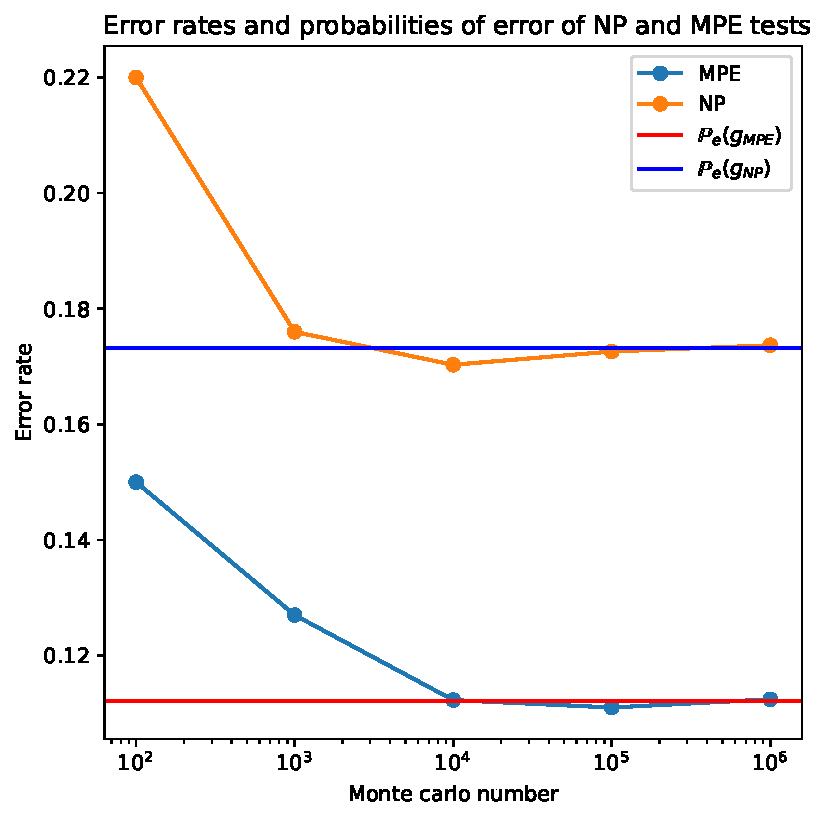
\includegraphics{Error_rate.pdf}
\end{figure}

D'après la figure obtenue ci-dessous, on voit que le test MPE a tendance à avoir un taux d'erreur et une probabilité d'erreur plus faibles par rapport au test NP. Dans le cadre de notre problème, le test MPE semble être le meilleur choix pour réduire les erreurs de classification.\\

6. On peut expliquer cette différence de performances par le fait que le test MPE cherche à minimiser la probabilité d'erreur pour choisir l'hypothèse la plus probable compte tenu des données et des probabilités a priori. En revanche, le test NP vise à contrôler strictement le taux d'erreur de Type I (faux positifs) avec le seuil tout en maximisant la puissance du test.
\end{document}
